\documentclass[tikz, margin=5mm]{standalone}
\usepackage[sfdefault,light]{roboto}
\usetikzlibrary{
	arrows,
	arrows.meta,
	chains,
	positioning,
	shapes,
	shapes.multipart,
	mindmap,
	fit,
	calc,
	intersections,
	backgrounds,
	scopes,
	matrix,
	shadows,
}
\definecolor{MyGreen}{HTML}{41B3A3}
\definecolor{MyOrange}{HTML}{E27D60}

\tikzset{every picture/.style={/utils/exec={\sffamily}}}
\begin{document}
    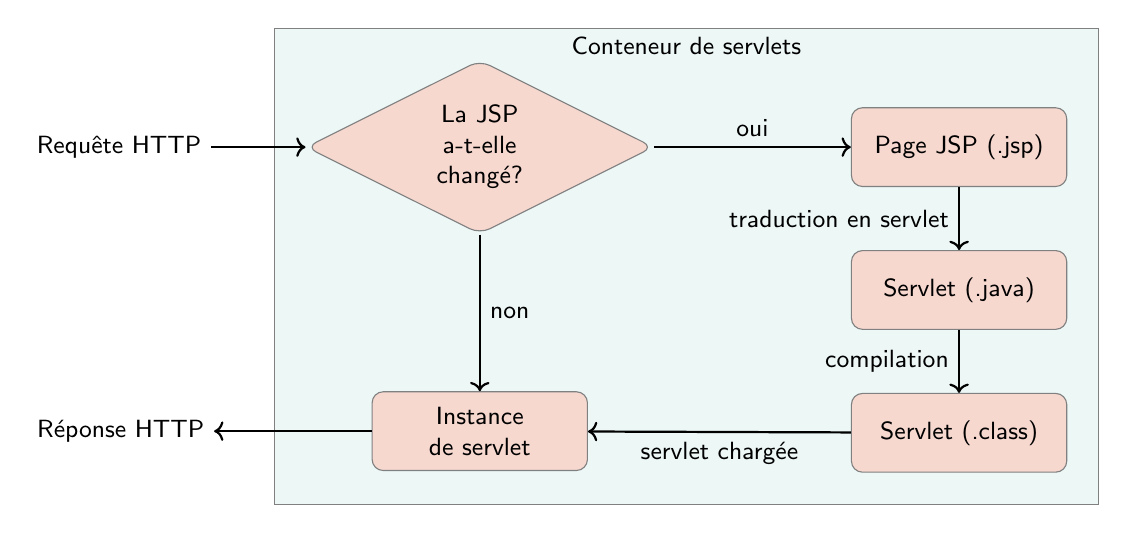
\begin{tikzpicture}	[
				every node/.style={align=center,draw=black!50,font=\small},
				block/.style={fill=MyOrange!30,rectangle,rounded corners,text width=25mm,minimum height=1cm},
			]
						
			\node (changed) [diamond,aspect=2,rounded corners,fill=MyOrange!30,text width=16mm] {La JSP a-t-elle changé?};
			\node (jsp) [block,right=2.5cm of changed] {Page JSP (.jsp)};
			\node (servlet) [block,below=0.8cm of jsp] {Servlet (.java)};
			\node (class) [block,below=0.8cm of servlet] {Servlet (.class)};
			\node (instance) [block,below=3.1cm of changed.center] {Instance de servlet};
			\node (request) [draw=none,left=1.2cm of changed] {Requête HTTP}; 			
			\node (reponse) [draw=none,left=2cm of instance] {Réponse HTTP}; 	
					
			\draw[->,thick] (request) -- (changed); 
			\draw[->,thick] (instance) -- (reponse); 
			\draw[->,thick] (changed) -- node[above,draw=none] {oui} (jsp); 
			\draw[->,thick] (changed) -- node[right,draw=none] {non} (instance);
			\draw[->,thick] (jsp) -- node[left,draw=none] {traduction en servlet} (servlet); 
			\draw[->,thick] (servlet) -- node[left,draw=none] {compilation} (class);
			\draw[->,thick] (class) -- node[below,draw=none] {servlet chargée} (instance); 
			
			\begin{scope}[on background layer]
				\node (conteneur) [
					rectangle, fill=MyGreen!10, inner sep=4mm,
					fit={(changed) (jsp) (servlet) (class) (instance)}
				] {};
				\node (cont) [below,draw=none] at (conteneur.north) {Conteneur de servlets};
			\end{scope}
		\end{tikzpicture}
\end{document}